\input{../utils/preamble}
\createdgmtitle{11}
%--------------------------------------------------------------------------------
\begin{document}
%--------------------------------------------------------------------------------
\begin{frame}
%\thispagestyle{empty}
\titlepage
\end{frame}
%=======
\begin{frame}{Evolution of GANs}
	\begin{figure}
		\centering
		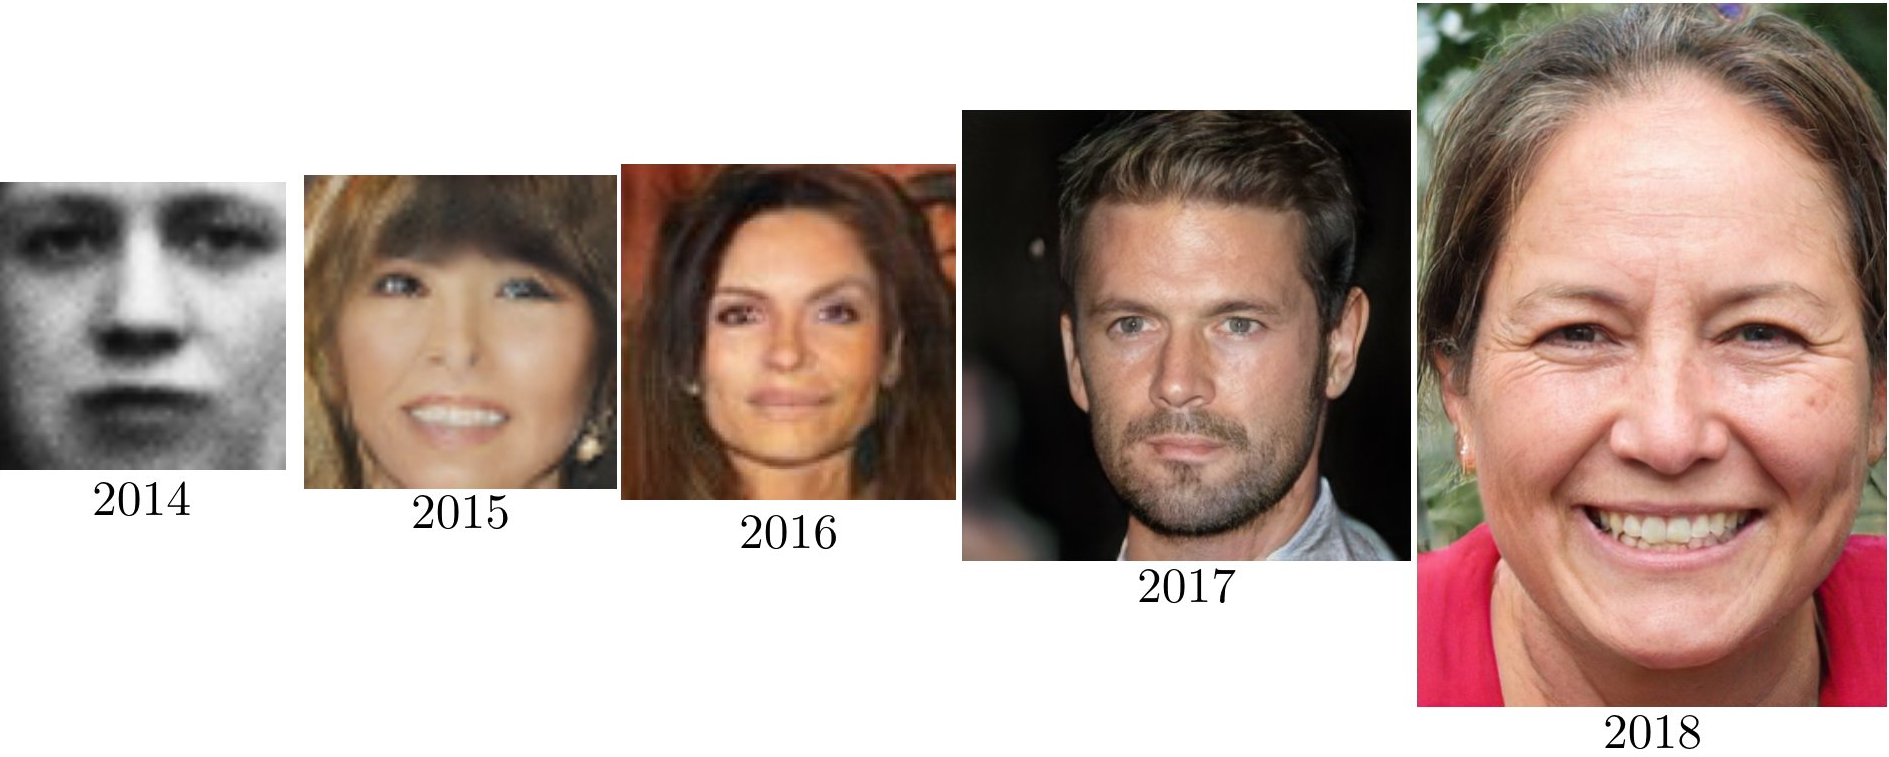
\includegraphics[width=\linewidth]{figs/gan_evolution}
	\end{figure}
	\begin{itemize}
		\item \textbf{Vanilla GAN} \href{https://arxiv.org/abs/1406.2661}{https://arxiv.org/abs/1406.2661}
		\item \textbf{DCGAN} \href{https://arxiv.org/abs/1511.06434}{https://arxiv.org/abs/1511.06434}
		\item \textbf{CoGAN} \href{https://arxiv.org/abs/1606.07536}{https://arxiv.org/abs/1606.07536}
		\item \textbf{ProGAN} \href{https://arxiv.org/abs/1710.10196}{https://arxiv.org/abs/1710.10196} 
		\item \textbf{StyleGAN} \href{https://arxiv.org/abs/1812.04948}{https://arxiv.org/abs/1812.04948}
	\end{itemize}
\end{frame}
%=======
\begin{frame}{Self-Attention GAN}
	\begin{itemize}
		\item Convolutional layers process the information in a local neighborhood.
		\item Using convolutional layers alone is computationally inefficient for modeling long-range dependencies in images.
	\end{itemize}
	\begin{figure}
		\centering
		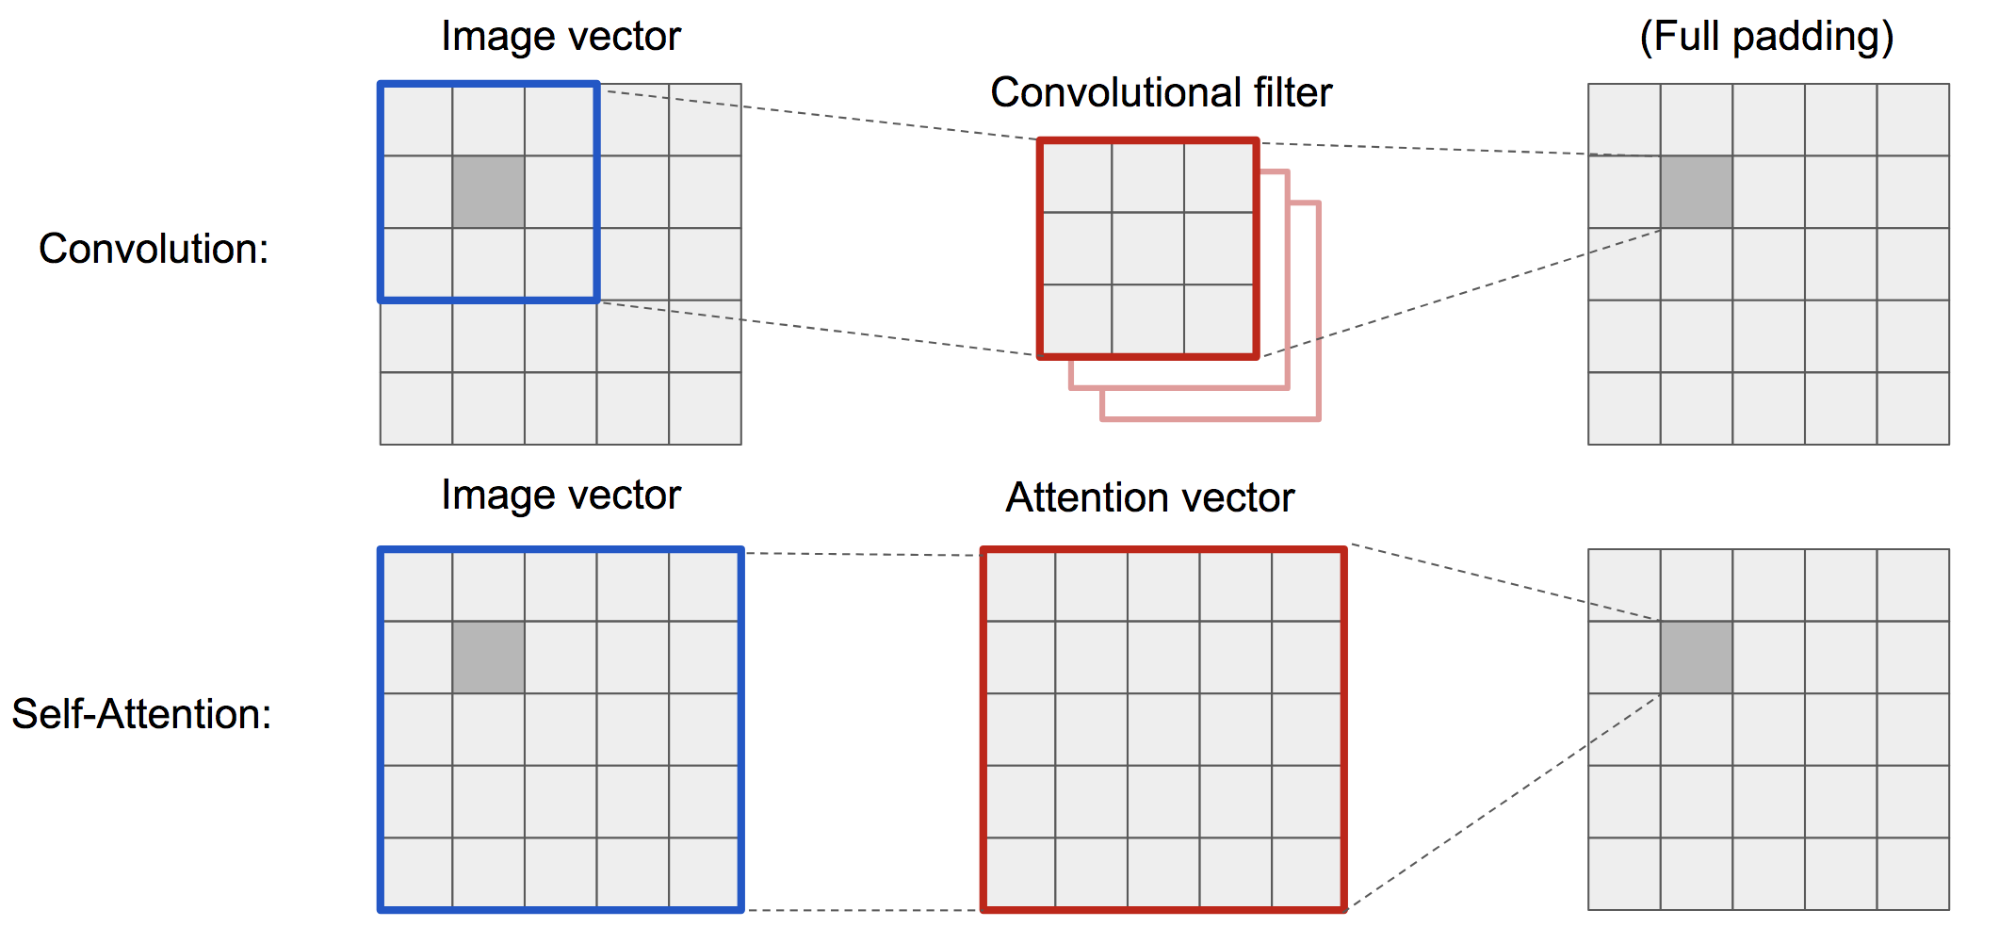
\includegraphics[width=0.9\linewidth]{figs/conv-vs-sa}
	\end{figure}
	\myfootnotewithlink{https://lilianweng.github.io/lil-log/2018/06/24/attention-attention.html}{image credit: https://lilianweng.github.io/lil-log/2018/06/24/attention-attention.html}
\end{frame}
%=======
\begin{frame}{Self-Attention GAN}
	\begin{figure}
		\centering
		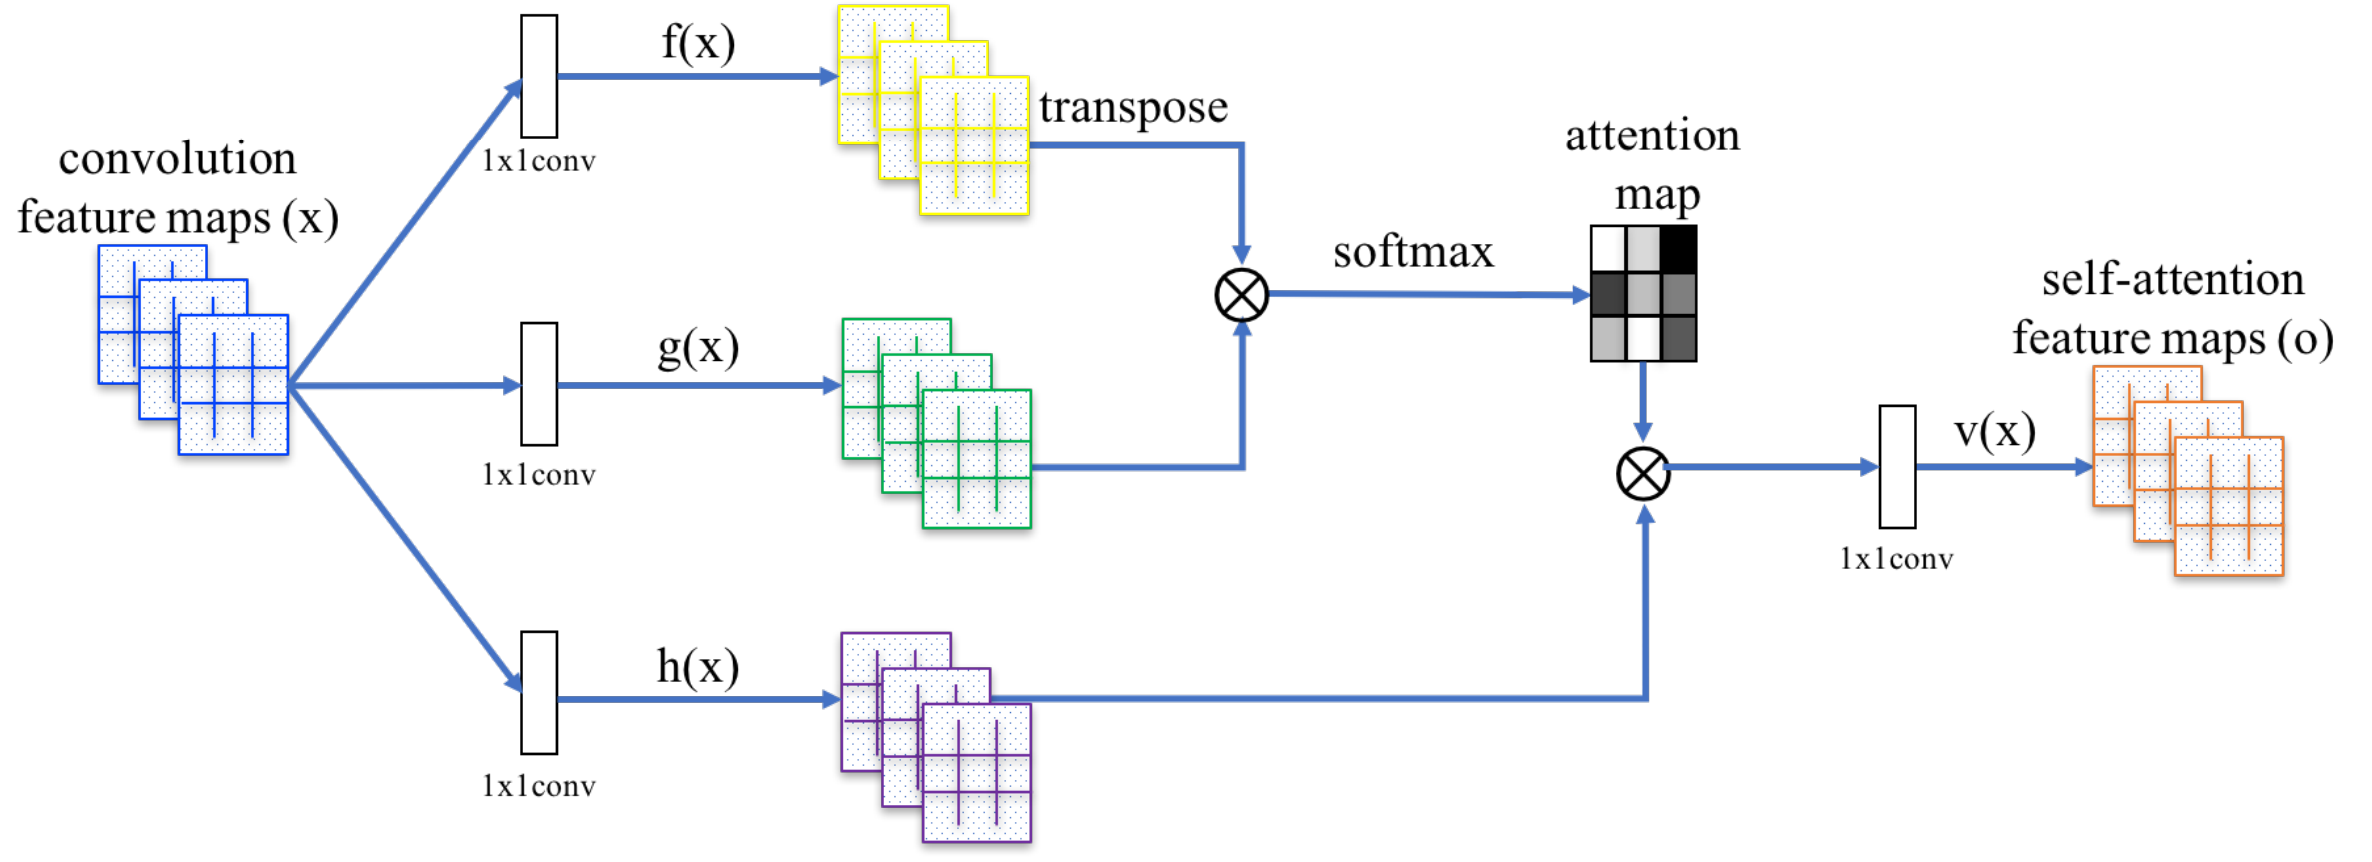
\includegraphics[width=0.9\linewidth]{figs/self-attention}
	\end{figure}
	\vspace{-0.2cm}
	\begin{itemize}
		\item $\bx$ -- feature vector for one feature location.
		\item $N$ -- number of feature locations.
	\end{itemize}
	\vspace{0.5cm}
	\[
		\mathbf{f}(\bx) = \bW_f(\bx), \quad \mathbf{g}(\bx) = \bW_g(\bx), \quad \mathbf{h}(\bx) = \bW_h(\bx), \quad \mathbf{v}(\bx) = \bW_v(\bx)
	\]
	\[
		s_{ij} = \mathbf{f}(\bx_i)^T \mathbf{g}(\bx_j), \quad a_{ij} = \frac{\exp{s_{ij}}}{\sum_{i=1}^N \exp{s_{ij}}}, \quad \textbf{o}_j = \textbf{v}\left( \sum_{i=1}^N a_{ij} \mathbf{h}(\bx_i) \right)
	\]
	\myfootnotewithlink{https://arxiv.org/abs/1805.08318}{Zhang H. et al. Self-Attention Generative Adversarial Networks, 2018}
\end{frame}
%=======
\begin{frame}{Self-Attention GAN}
	\begin{block}{Technical Details}
		\begin{itemize}
			\item Hinge loss for training.
			\item Spectral Normalization in both the generator and the discriminator.
			\item Separate learning rates for the generator and the discriminator.
		\end{itemize}
	\end{block}
	\begin{figure}
		\centering
		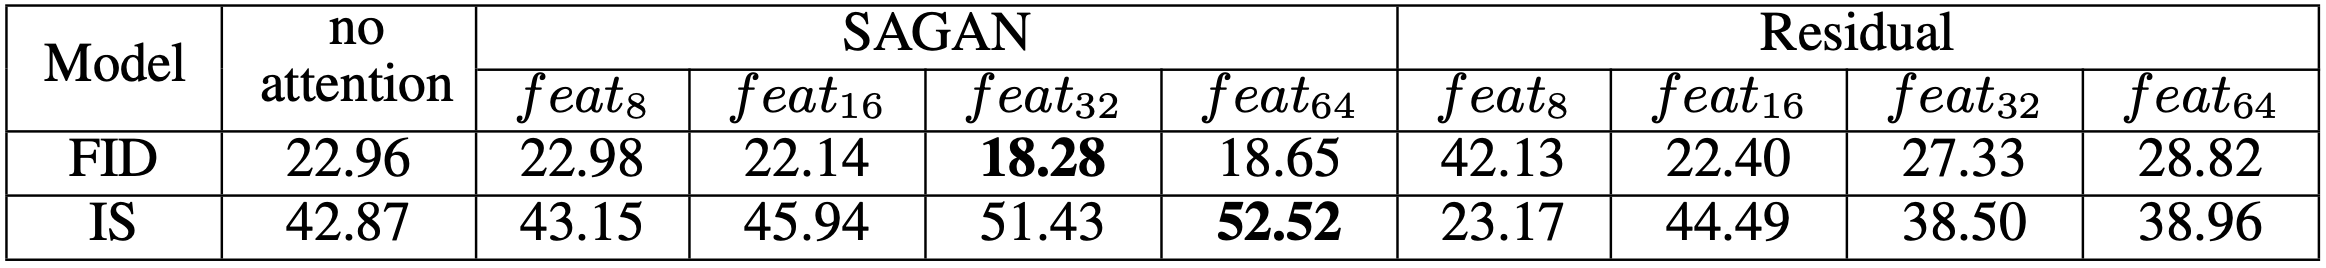
\includegraphics[width=\linewidth]{figs/sa_results1}
	\end{figure}
	\begin{figure}
		\centering
		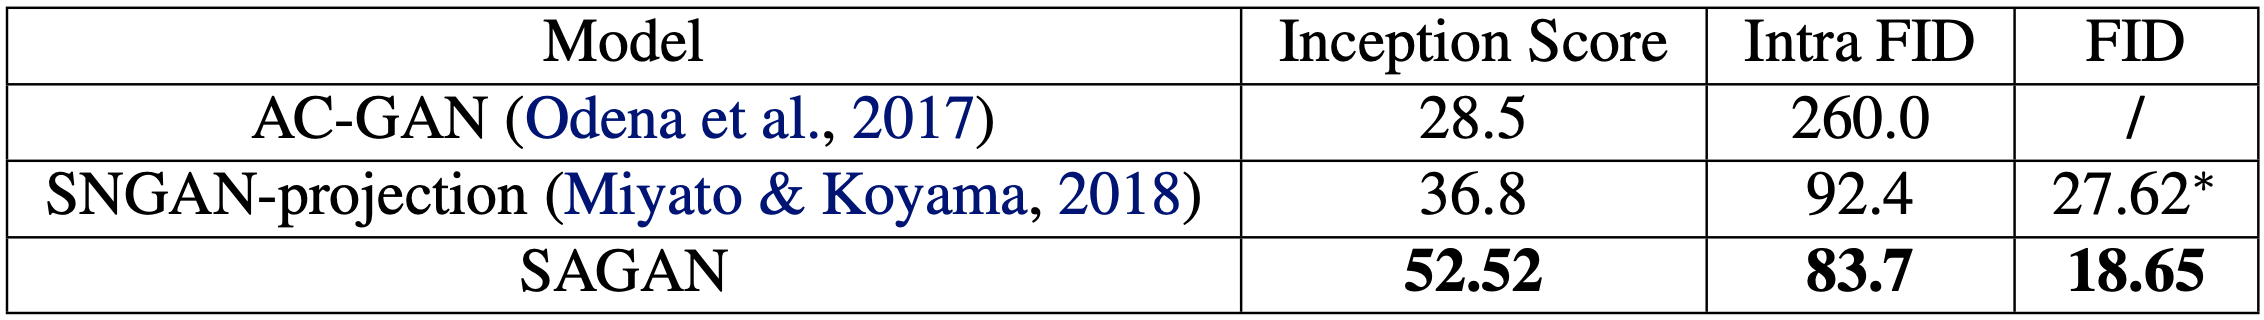
\includegraphics[width=\linewidth]{figs/sa_results2}
	\end{figure}

	\myfootnotewithlink{https://arxiv.org/abs/1805.08318}{Zhang H. et al. Self-Attention Generative Adversarial Networks, 2018}
\end{frame}
%=======
\begin{frame}{Self-Attention GAN}
	\begin{block}{Visualization of attention maps}
		\begin{figure}
			\centering
			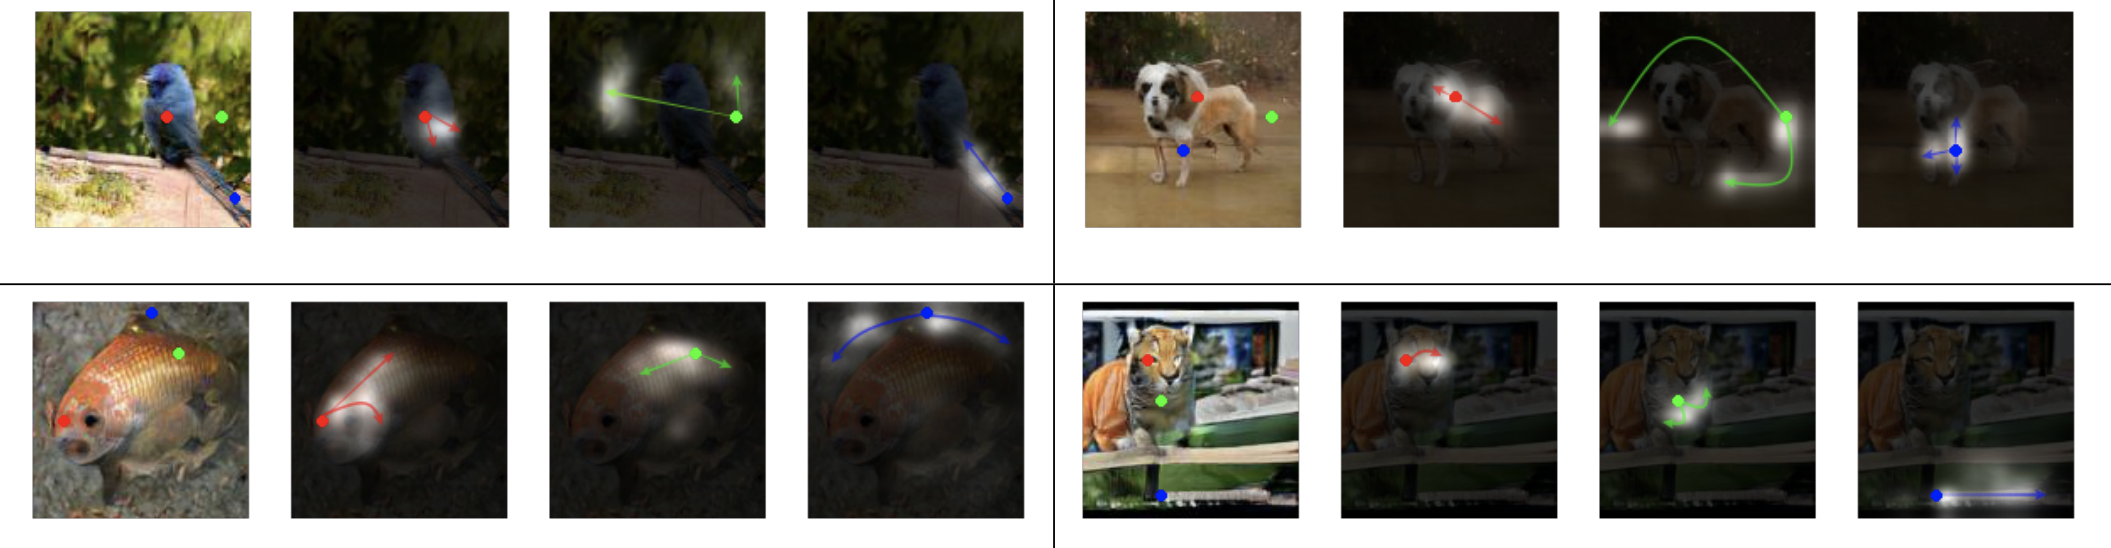
\includegraphics[width=\linewidth]{figs/sa_maps}
		\end{figure}
	\end{block}

	\myfootnotewithlink{https://arxiv.org/abs/1805.08318}{Zhang H. et al. Self-Attention Generative Adversarial Networks, 2018}
\end{frame}
%=======
\begin{frame}{BigGAN}
	\begin{block}{Model description}
		\begin{itemize}
			\item Self-Attention GAN baseline.
			\item Class-conditional generator.
			\item Increasing batch size gives tremendous benefit (allows to cover more modes).
			\item Increasing model size is helpful (wider helps as much as deeper).
			\item Hinge loss for training.
			\item Orthogonal regularization for smoothness the generator output.
			\item Truncation trick for balancing between diversity and fidelity.
		\end{itemize}
	\end{block}
	\vspace{0.5cm}

	\myfootnotewithlink{https://arxiv.org/abs/1809.11096}{Brock A., Donahue J., Simonyan K. Large Scale GAN Training for High Fidelity Natural Image Synthesis, 2018}
\end{frame}
%=======
\begin{frame}{BigGAN}
	\begin{itemize}
		\item \textbf{Orthogonal regularization}
		\[
		\| \bW^T \bW - \bI \|^2 \quad \Rightarrow \| \bW^T \bW - \text{diag}(\bW^T \bW) \|^2
		\]
		\item \textbf{Truncation trick.} Coordinates of samples $\bz \sim \cN(0, \bI)$ which fall outside a predefined range are resampled to fall inside that range.
	\end{itemize}
	\begin{figure}
		\centering
		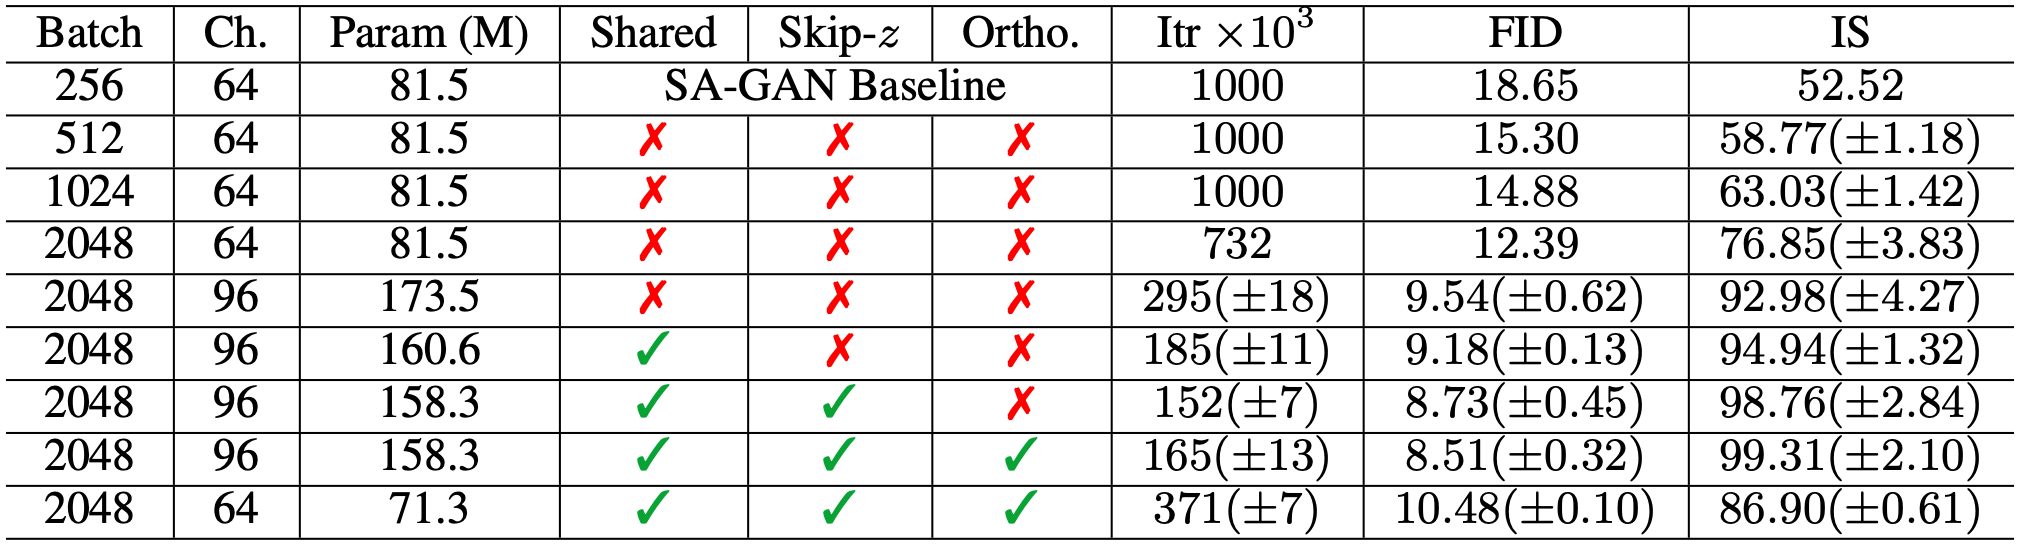
\includegraphics[width=\linewidth]{figs/biggan_results}
	\end{figure}
	
	\myfootnotewithlink{https://arxiv.org/abs/1809.11096}{Brock A., Donahue J., Simonyan K. Large Scale GAN Training for High Fidelity Natural Image Synthesis, 2018}
\end{frame}
%=======
\begin{frame}{BigGAN}
	\begin{block}{Samples (512x512)}
		\begin{figure}
			\centering
			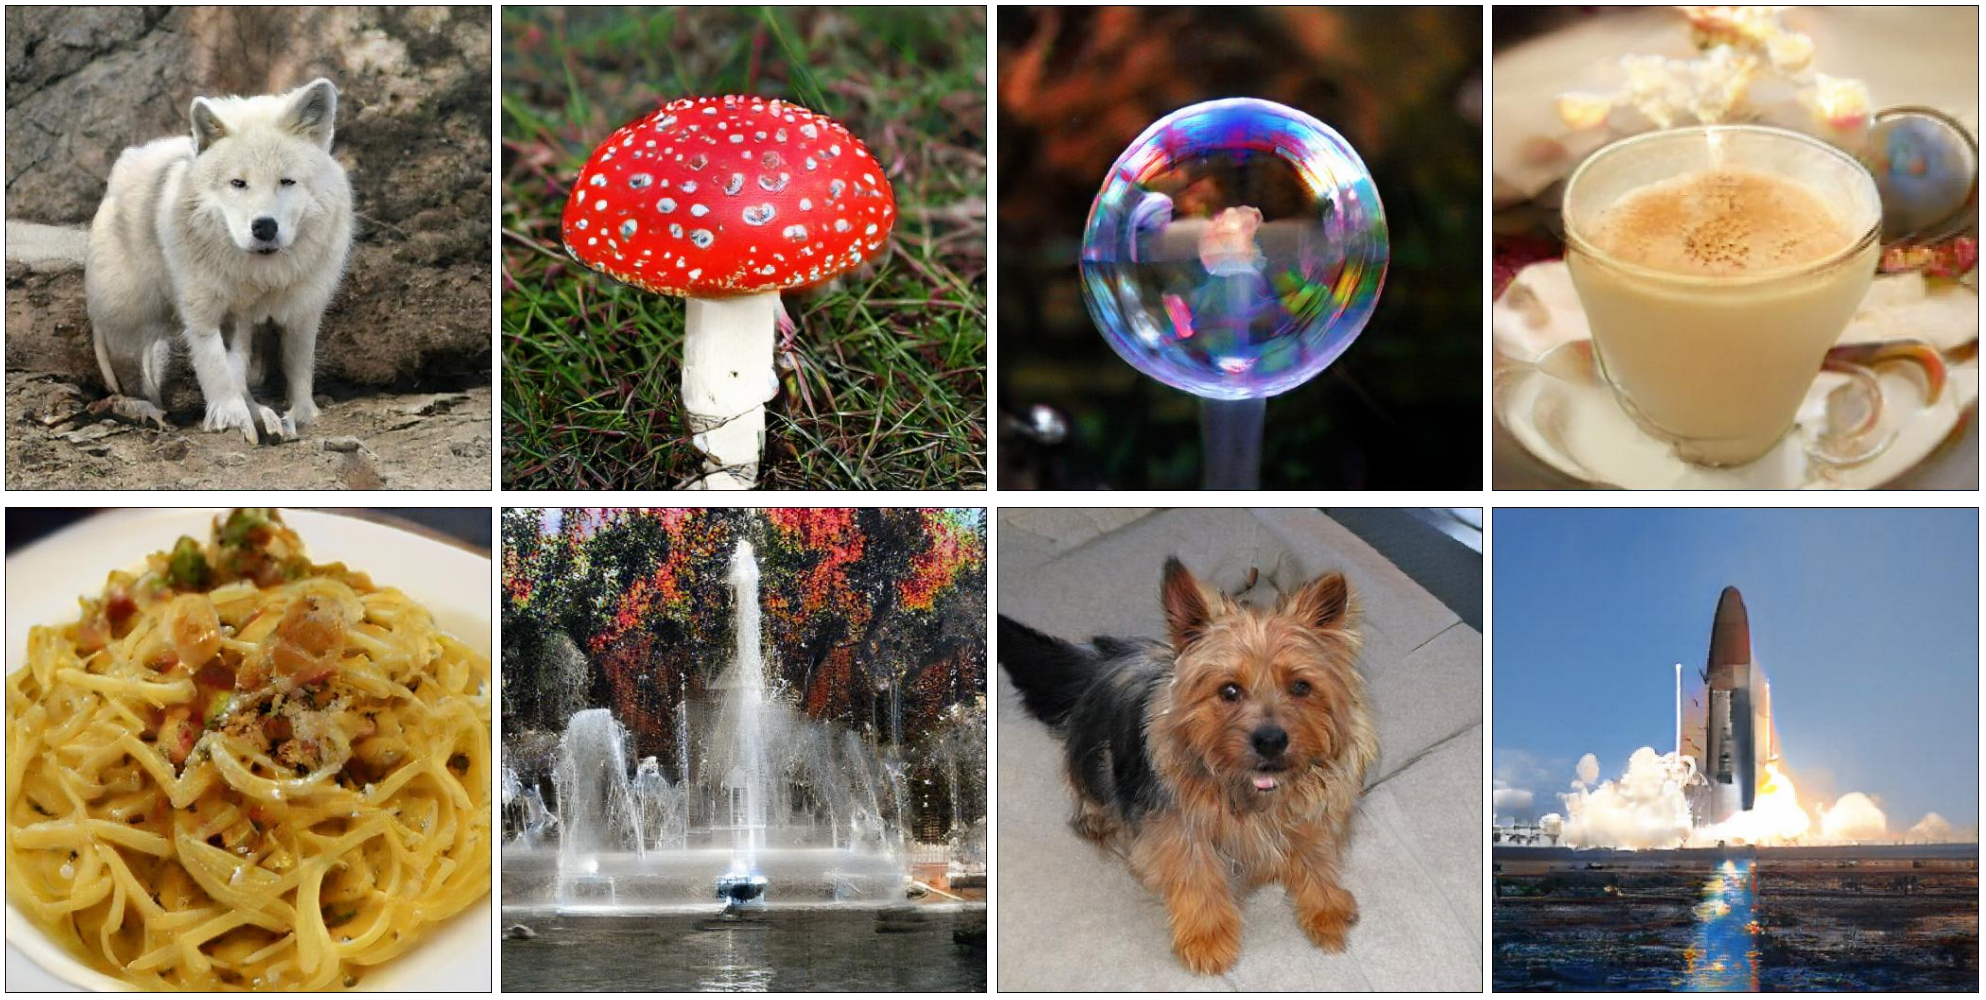
\includegraphics[width=\linewidth]{figs/biggan_samples}
		\end{figure}
	\end{block}
	
	\myfootnotewithlink{https://arxiv.org/abs/1809.11096}{Brock A., Donahue J., Simonyan K. Large Scale GAN Training for High Fidelity Natural Image Synthesis, 2018}
\end{frame}
%=======
\begin{frame}{BigGAN}
	\begin{block}{Interpolations}
		\begin{figure}
			\centering
			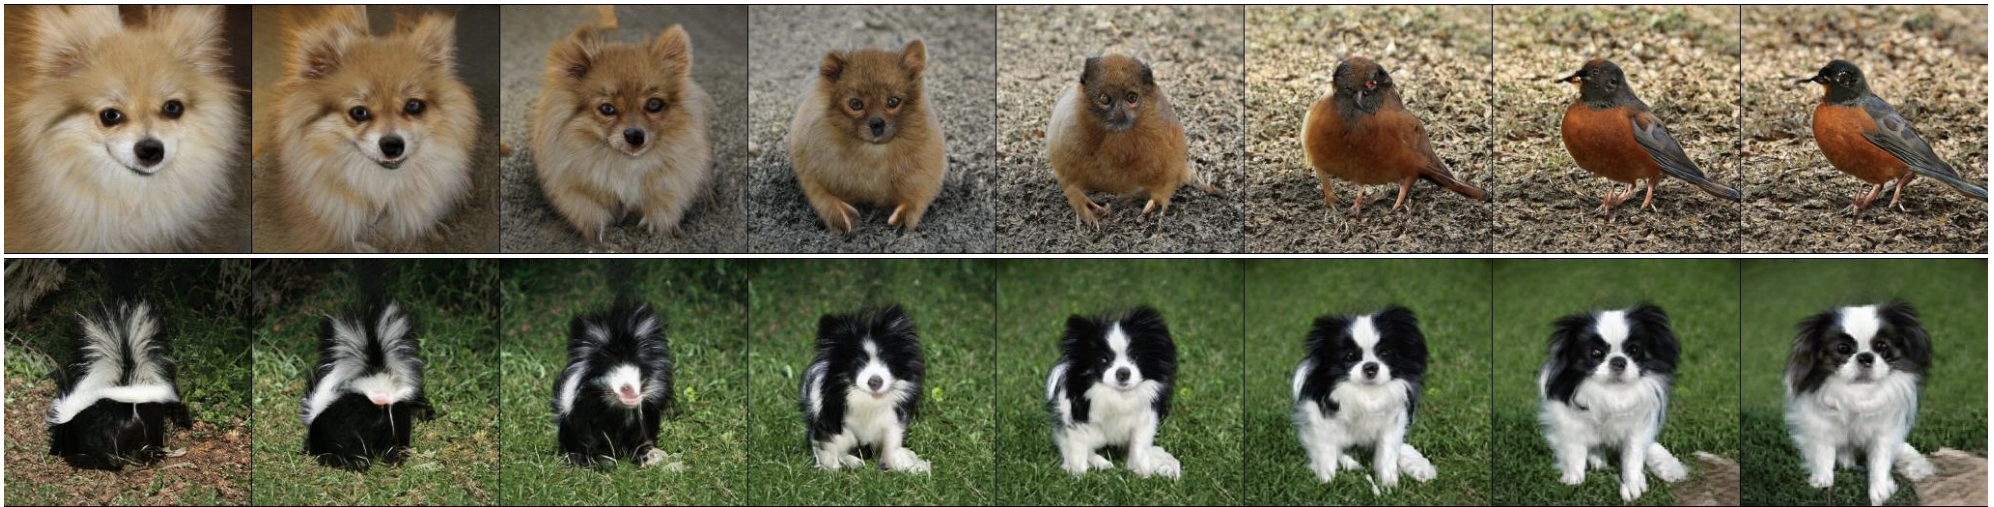
\includegraphics[width=\linewidth]{figs/biggan_interpolations}
		\end{figure}
	\end{block}
	\myfootnotewithlink{https://arxiv.org/abs/1809.11096}{Brock A., Donahue J., Simonyan K. Large Scale GAN Training for High Fidelity Natural Image Synthesis, 2018}
\end{frame}
%=======
\begin{frame}{Progressive Growing GAN}
	\begin{block}{Problems with HR image generation}
		\begin{itemize}
			\item Disjoint manifolds $\Rightarrow$ gradient problem.
			\item Small minibatch $\Rightarrow$ training instability.
		\end{itemize}
	\end{block}
	\begin{block}{Solution}
		Grow both the generator and discriminator progressively, starting from LR images, and add new layers that introduce higher-resolution details as the training progresses. 
		\begin{itemize}
			\item Train GAN which generate 4x4 images (just 2 convolutions for G and D).
			\item Add upsampling layers to G, downsampling layers to D.
			\item Train GAN which generate 8x8 images.
			\item etc.
		\end{itemize}
	\end{block}
	
	\myfootnotewithlink{https://arxiv.org/abs/1710.10196}{Karras T. et al. Progressive Growing of GANs for Improved Quality, Stability, and Variation, 2017}
\end{frame}
\begin{frame}{Progressive Growing GAN}
	\begin{figure}
		\centering
		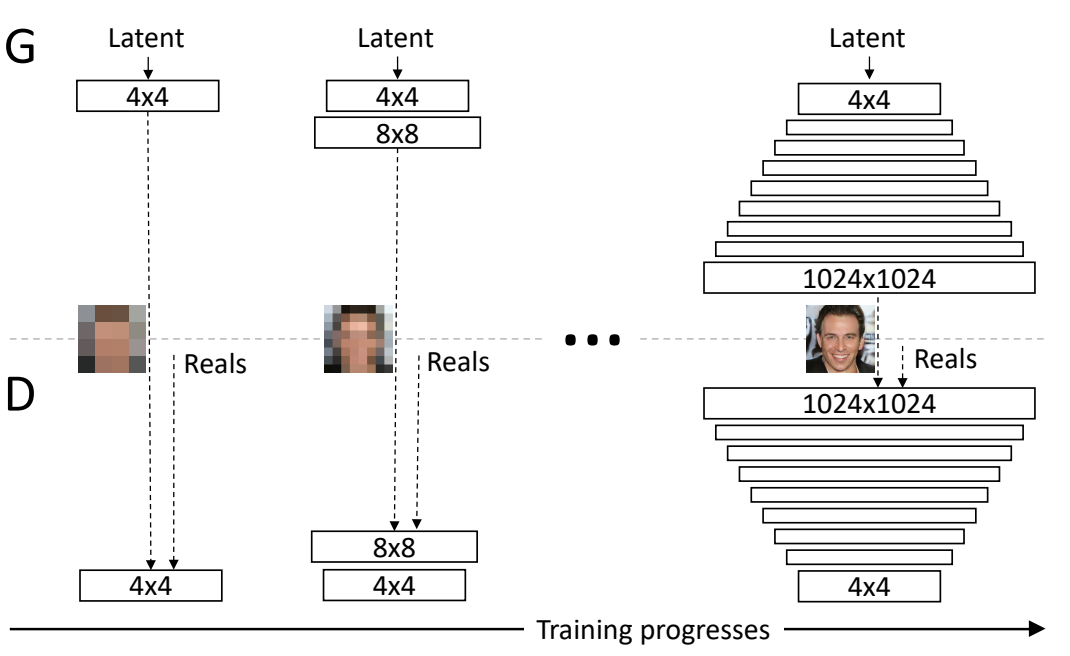
\includegraphics[width=0.8\linewidth]{figs/pggan_arch}
	\end{figure}
	\begin{figure}
		\centering
		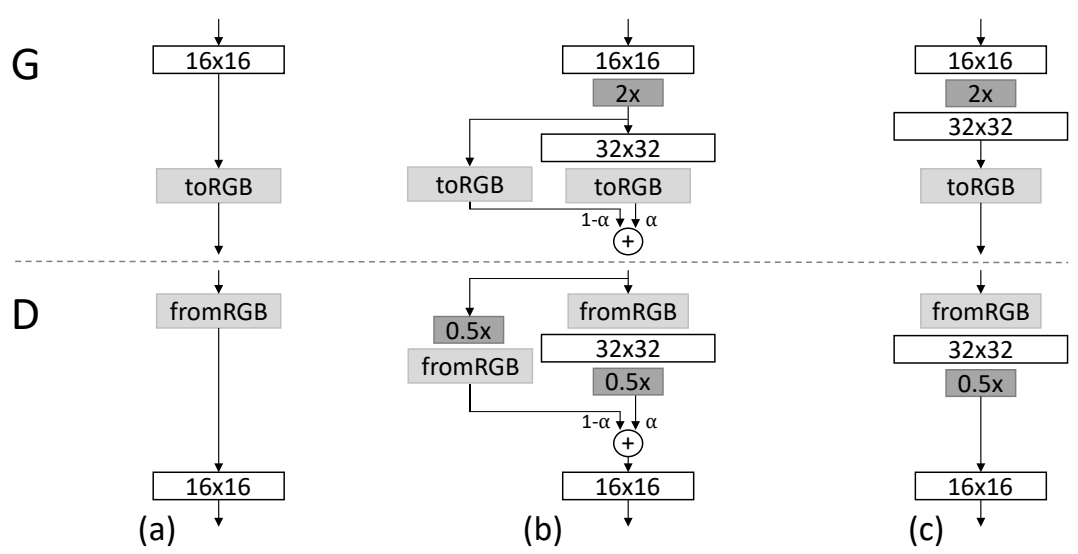
\includegraphics[width=0.6\linewidth]{figs/pggan_fadein}
	\end{figure}

	\myfootnotewithlink{https://arxiv.org/abs/1710.10196}{Karras T. et al. Progressive Growing of GANs for Improved Quality, Stability, and Variation, 2017}
\end{frame}
%=======
\begin{frame}{Progressive Growing GAN}
	\begin{block}{Samples (1024x1024)}
		\begin{figure}
			\centering
			\includegraphics[width=\linewidth]{figs/pggan_samples}
		\end{figure}
	\end{block}

	\myfootnotewithlink{https://arxiv.org/abs/1710.10196}{Karras T. et al. Progressive Growing of GANs for Improved Quality, Stability, and Variation, 2017}
\end{frame}
%=======
\begin{frame}{StyleGAN}
	\begin{itemize}
		\item Generating of HR images is hard.
		\item Progressive growing greatly simplifies the task.
		\item The ability to control specific features of the generated image is very limited.
	\end{itemize}
	\begin{block}{Face image features}
		\begin{itemize}
			\item Coarse (pose, general hair style, face shape). Resolution $4^2 - 8^2$.
			\item Middle (finer facial features, hair style, eyes open/closed). Resolution $16^2 - 32^2$.
			\item Fine (color scheme (eye, hair and skin) and micro features). Resolution $64^2 - 1024^2$.
		\end{itemize}
	\end{block}
	\myfootnotewithlink{https://arxiv.org/abs/1812.04948}{Karras T., Laine S., Aila T. A Style-Based Generator Architecture for Generative Adversarial Networks, 2018}
\end{frame}
%=======
\begin{frame}{StyleGAN}
	\begin{block}{Step 1: Mapping Network}
		\begin{itemize}
			\item Generator input is likely to be \textbf{disentangled}.  Each component of input vector $\bz$ should be responsible for one generative factor.
			\item Mapping network $f: \cZ \rightarrow \cW$ is used to reduce correlations between components of~$\bz$.
		\end{itemize}
		\begin{minipage}[t]{0.6\columnwidth}
			\begin{figure}
				\centering
				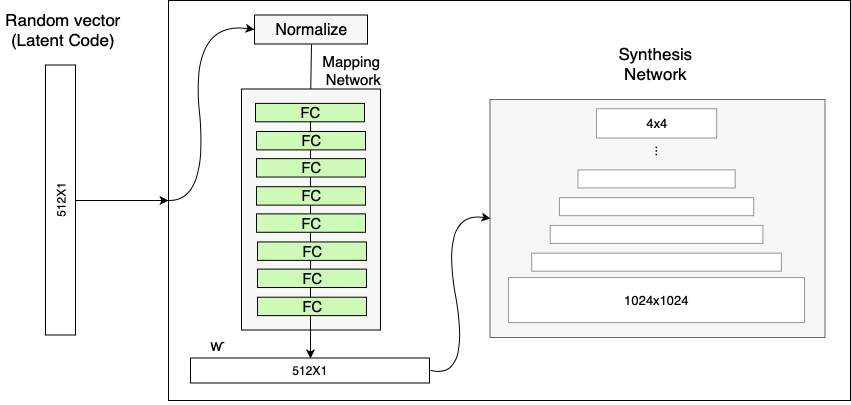
\includegraphics[width=0.98\linewidth]{figs/stylegan_mapping}
			\end{figure}
		\end{minipage}%
		\begin{minipage}[t]{0.38\columnwidth}
			\begin{figure}
				\centering
				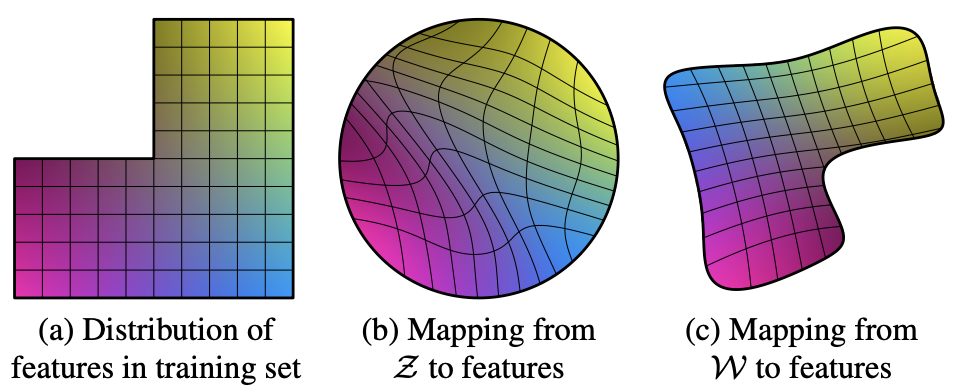
\includegraphics[width=1.0\linewidth]{figs/stylegan_curved}
			\end{figure}
		\end{minipage}
	\vspace{0.3cm}
	\end{block}

	\myfootnotewithlink{https://arxiv.org/abs/1812.04948}{Karras T., Laine S., Aila T. A Style-Based Generator Architecture for Generative Adversarial Networks, 2018}
\end{frame}
%=======
\begin{frame}{StyleGAN}
	\begin{block}{Step 2: Style modulation}
		\begin{itemize}
			\item Adaptive Instance Normalization transfers the $\bw$ vector to the synthesis Network.
			\item The module is added to each resolution to define the visual expression of the features.
		\end{itemize}
		\begin{figure}
			\centering
			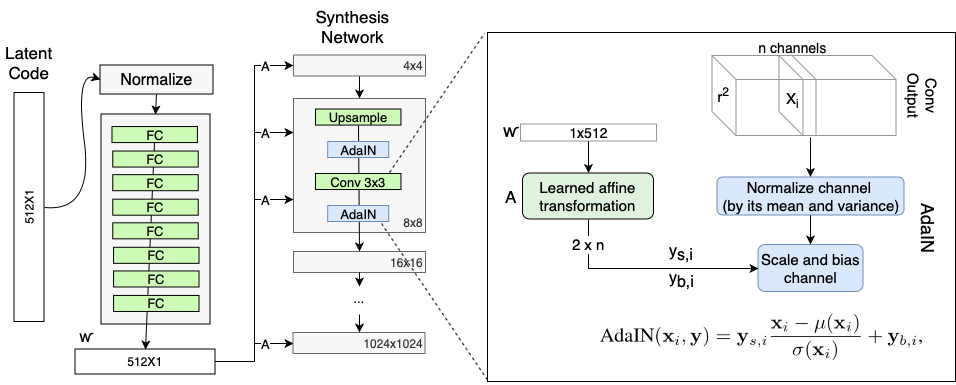
\includegraphics[width=1.0\linewidth]{figs/stylegan_adain}
		\end{figure}
	\end{block}

	\myfootnotewithlink{https://arxiv.org/abs/1812.04948}{Karras T., Laine S., Aila T. A Style-Based Generator Architecture for Generative Adversarial Networks, 2018}
\end{frame}
%=======
\begin{frame}{StyleGAN}
	\begin{block}{Step 3: Remove traditional input}
		Mapping network provides stochasticity to different stages of the synthesis network. Input of the synthesis network is a trainable vector.
		\begin{figure}
			\centering
			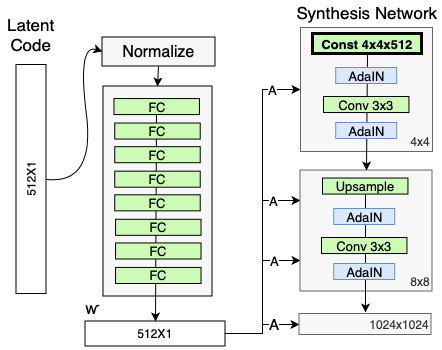
\includegraphics[width=0.55\linewidth]{figs/stylegan_input}
		\end{figure}
	\end{block}

	\myfootnotewithlink{https://arxiv.org/abs/1812.04948}{Karras T., Laine S., Aila T. A Style-Based Generator Architecture for Generative Adversarial Networks, 2018}
\end{frame}
%=======
\begin{frame}{StyleGAN}
	\begin{block}{Step 4: Stochastic variation}
		Inject random noise to add small aspects, such as freckles, exact placement of hairs, wrinkles, features which make the image more realistic and increase the variety of outputs.
		\begin{figure}
			\centering
			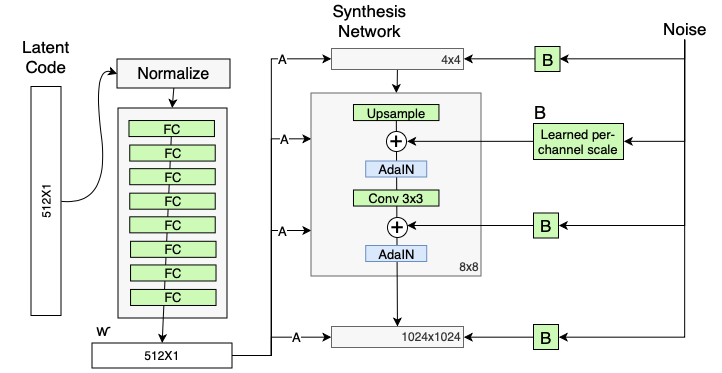
\includegraphics[width=0.9\linewidth]{figs/stylegan_noise}
		\end{figure}
	\end{block}

	\myfootnotewithlink{https://arxiv.org/abs/1812.04948}{Karras T., Laine S., Aila T. A Style-Based Generator Architecture for Generative Adversarial Networks, 2018}
\end{frame}
%=======
\begin{frame}{StyleGAN}
	\begin{block}{Step 4: Style Mixing}
		\vspace{-0.33cm}
		\begin{figure}
			\centering
			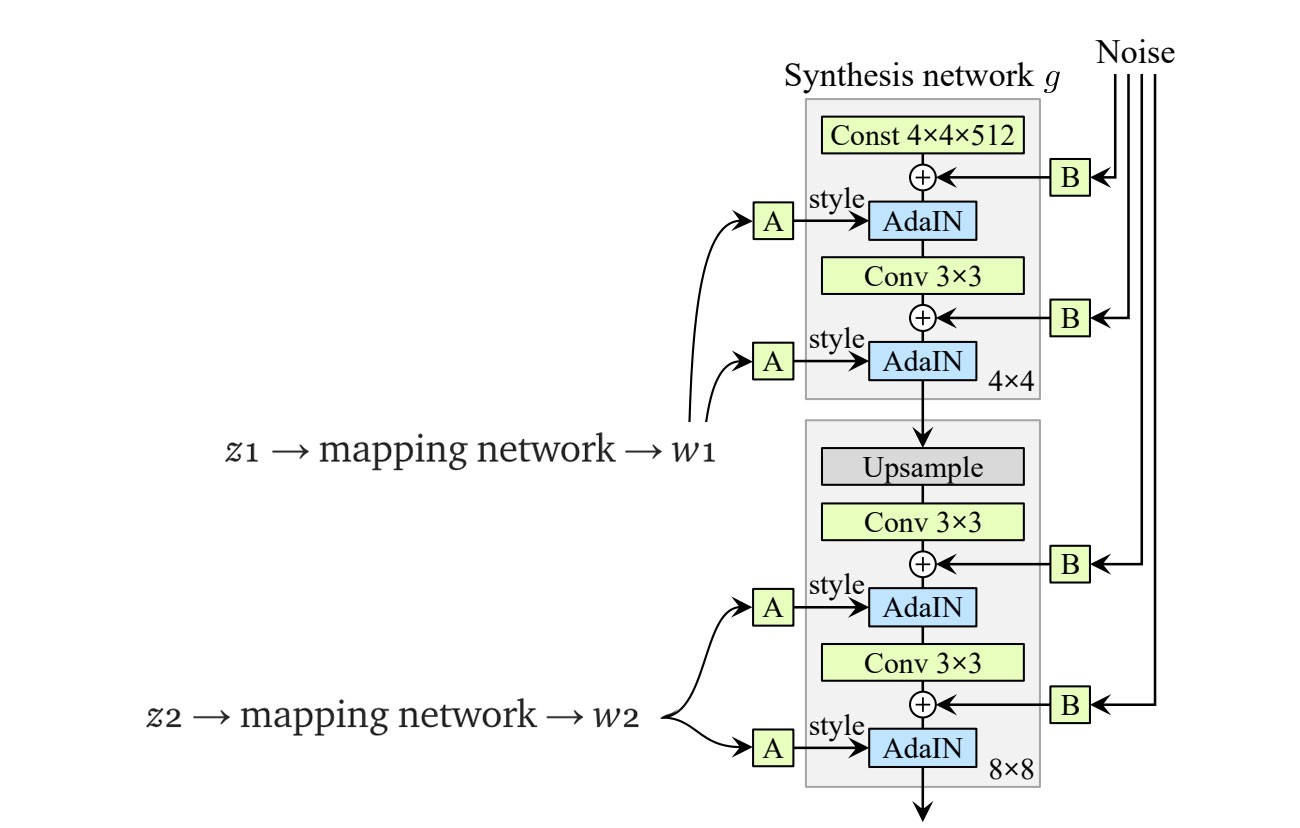
\includegraphics[width=0.8\linewidth]{figs/stylegan_mix_reg}
		\end{figure}
	\begin{itemize}
		\item Makes different levels of synthesis network to be independent.
		\item Allows to couple diffirent styles.
	\end{itemize}
	\end{block}

	\myfootnotewithlink{https://arxiv.org/abs/1812.04948}{Karras T., Laine S., Aila T. A Style-Based Generator Architecture for Generative Adversarial Networks, 2018}
\end{frame}
%=======
\begin{frame}{StyleGAN}
	\begin{figure}
		\centering
		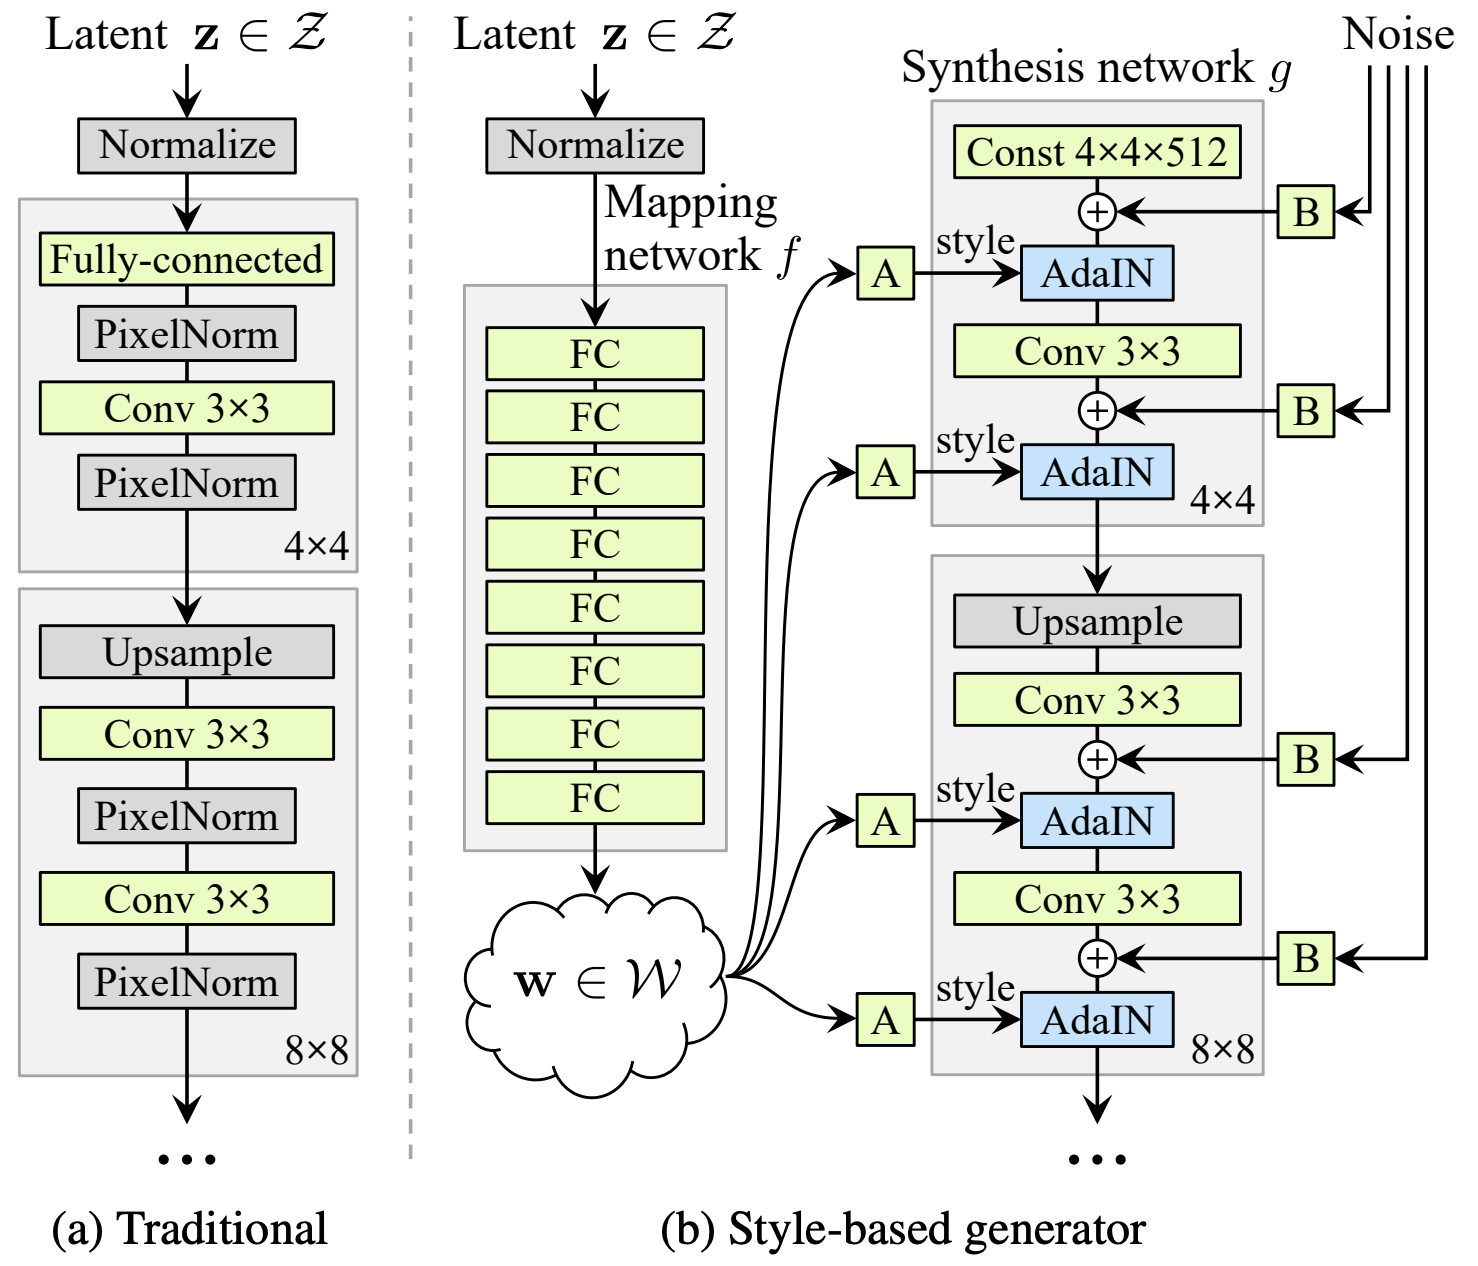
\includegraphics[width=0.8\linewidth]{figs/stylegan_scheme}
	\end{figure}

	\myfootnotewithlink{https://arxiv.org/abs/1812.04948}{Karras T., Laine S., Aila T. A Style-Based Generator Architecture for Generative Adversarial Networks, 2018}
\end{frame}
%=======
\begin{frame}{StyleGAN}
	\begin{block}{Truncation trick}
		\vspace{-0.2cm}
		\[
			\bw' = \hat{\bw} - \psi \cdot (\bw - \hat{\bw}), \quad \hat{\bw} = \bbE_{\bz} p(f(\bz))
		\]
		\vspace{-0.2cm}
		\begin{itemize}
			\item Constant $\psi$ is a tradeoff between diversity and fidelity. 
			\item $\psi=0.7$ is used for most of the results.
			\item Truncation is done only at the low-resolution layers.
		\end{itemize}
		\begin{figure}
			\centering
			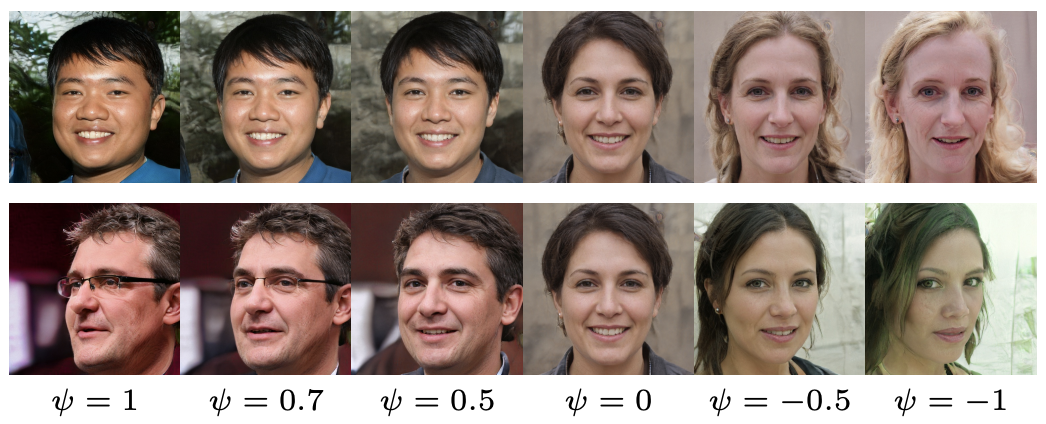
\includegraphics[width=0.8\linewidth]{figs/stylegan_truncation}
		\end{figure}
	\end{block}

	\myfootnotewithlink{https://arxiv.org/abs/1812.04948}{Karras T., Laine S., Aila T. A Style-Based Generator Architecture for Generative Adversarial Networks, 2018}
\end{frame}
%=======
\begin{frame}{StyleGAN}
	\begin{block}{Results}
		\vspace{-0.2cm}
		\begin{figure}
			\centering
			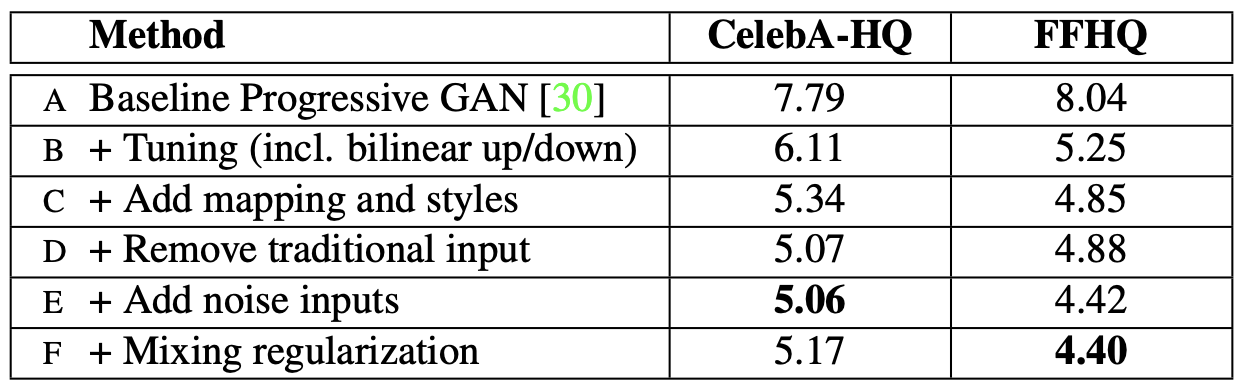
\includegraphics[width=0.6\linewidth]{figs/stylegan_results}
		\end{figure}
	\vspace{-0.3cm}
	\end{block}
	\begin{block}{Samples (1024x1024)}
		\begin{figure}
			\centering
			\includegraphics[width=0.8\linewidth]{figs/stylegan_samples}
		\end{figure}
	\vspace{-0.1cm}
	\end{block}

	\myfootnotewithlink{https://arxiv.org/abs/1812.04948}{Karras T., Laine S., Aila T. A Style-Based Generator Architecture for Generative Adversarial Networks, 2018}
\end{frame}
%=======
\begin{frame}{StyleGAN}
		\begin{figure}
			\centering
			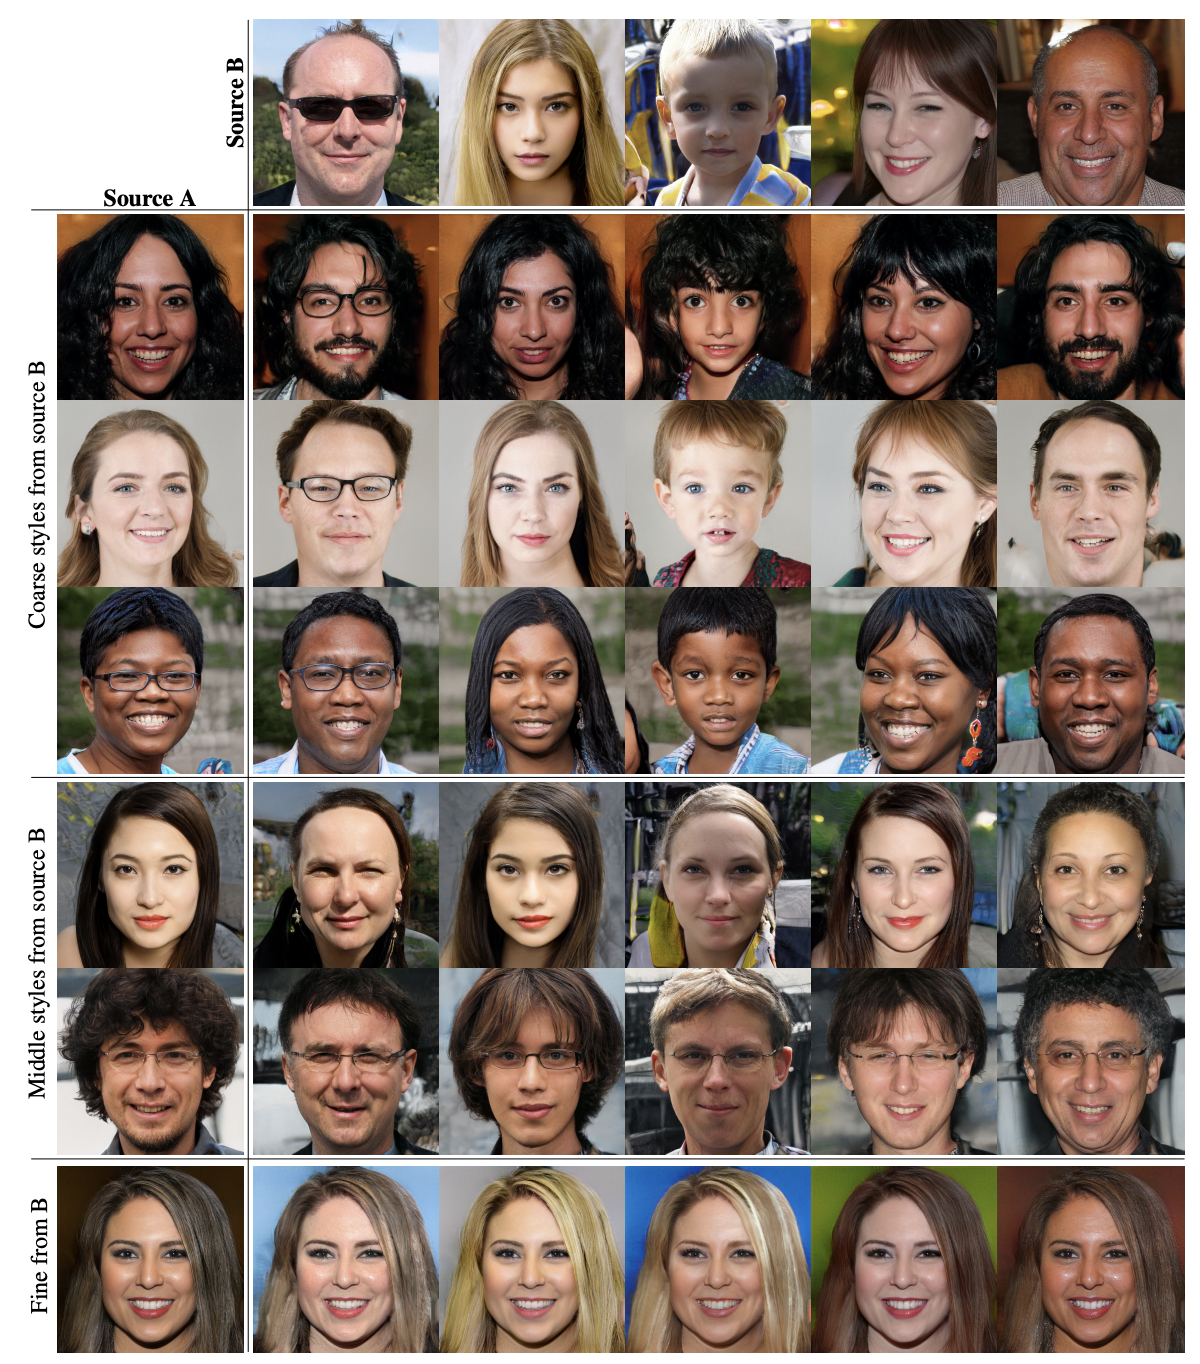
\includegraphics[width=0.6\linewidth]{figs/stylegan_mix}
		\end{figure}

	\myfootnotewithlink{https://arxiv.org/abs/1812.04948}{Karras T., Laine S., Aila T. A Style-Based Generator Architecture for Generative Adversarial Networks, 2018}
\end{frame}
%=======
\begin{frame}{Summary}
\end{frame}
%=======
\end{document} 